%En-tête classique
\documentclass[11pt,a4paper]{article}
\usepackage[french]{babel}
\usepackage[utf8]{inputenc}
\usepackage[T1]{fontenc}
\usepackage{listings}
\usepackage{xcolor}

%%%% Requis : police Fira Sans + compilation xetex !!! %%%%

%Packages ams
\usepackage[intlimits]{amsmath}
\usepackage{amsfonts}
\usepackage{amssymb}
\usepackage{amsthm}
\usepackage{stmaryrd}

%Fonction indicatrice
\usepackage[upint]{newtxmath}

% réglages font Fira Sans (ATTENTION : XeTex REQUIS !!)
%\usepackage{mathspec}
%\setmainfont[BoldFont=Fira Sans Bold]{Fira Sans}
%\setmathsfont(Digits,Latin)[Numbers={Lining,Proportional}]{Fira Sans}
%\setmathrm[]{Fira Sans}
%\setmathbb[]{Fira Sans Bold}
%\setmonofont[Scale=1]{Ubuntu Mono}

%police perso Fira sans - attention compilation par Latex
\usepackage[default,regular,bold]{sourceserifpro}


%mise en page
\usepackage{multicol}
\usepackage[hidelinks]{hyperref}
\usepackage{fancyhdr}
\usepackage{tabularx} %personalisation des tableaux
\usepackage{graphicx} %importation d'images
\usepackage{enumitem} %personalisation de itemize/enumerate
\usepackage{array} %extension de array/tableaux
\usepackage[left=2cm,right=2cm,top=2cm,bottom=2cm]{geometry} %mise en page
\pagestyle{plain}
\usepackage{lastpage}

%extensions requises par bclogo
\usepackage{xkeyval}
\usepackage{ifthen}
\usepackage{ifpdf}
\usepackage{etoolbox}
\usepackage[tikz]{bclogo}

%paramètres de bclogo
\presetkeys{bclogo}{ombre=true,epOmbre=0.25}{}
\newcommand{\eb}{\end{bclogo}}

%paramétrage bclogo définition
\newcounter{definition}
\setcounter{definition}{0}
\newcommand{\bd}[1]{\addtocounter{definition}{1} \begin{bclogo}[logo=\bcinfo ,sousTitre=#1,nobreak=true]{Définition \thedefinition}}

%paramétrage bclogo théorème
\newcounter{theoreme}
\setcounter{theoreme}{0}
\newcommand{\bt}[1]{\addtocounter{theoreme}{1} \begin{bclogo}[logo=\bctrombone ,arrondi=0.1,sousTitre=#1,nobreak=true]{Théorème \thetheoreme}}

%paramétrage bclogo théorème-définition
\newcounter{deftheo}
\setcounter{deftheo}{0}
\newcommand{\btd}[1]{\addtocounter{deftheo}{1} \begin{bclogo}[logo=\bctrombone ,arrondi=0.1,sousTitre=#1,nobreak=true]{Théorème - Définition \thedeftheo}}

%paramétrage bclogo proposition
\newcounter{proposition}
\setcounter{proposition}{0}
\newcommand{\bp}[1]{\addtocounter{proposition}{1} \begin{bclogo}[logo=\bclampe, sousTitre=#1]{Proposition \theproposition}}

%paramétrage bclogo proposition-définition
\newcommand{\bpd}[1]{\begin{bclogo}[logo=\bctrombone ,arrondi=0.1,sousTitre=#1,nobreak=true]{Proposition - Définition}}

%paramétrage bclogo lemme
\newcounter{lemme}
\setcounter{lemme}{0}
\newcommand{\bl}[1]{\addtocounter{lemme}{1} \begin{bclogo}[logo=\bclampe, sousTitre=#1]{Lemme \thelemme}}

%paramétrage bclogo corollaire
\newcounter{corollaire}
\setcounter{corollaire}{0}
\newcommand{\bcq}[1]{\addtocounter{corollaire}{1} \begin{bclogo}[noborder=true,sousTitre=#1]{Corollaire \thecorollaire}}

%paramétrage bclogo méthode, preuve, remarque, exemple, attention, notations
\newcommand{\bm}[1]{\begin{bclogo}[logo=\bcoutil ,noborder=true,sousTitre=#1]{Méthode}}
\newcommand{\bdm}{\begin{bclogo}[logo=\bcloupe ,margeG=1,noborder=true]{Preuve}}
\newcommand{\br}{\begin{bclogo}[margeG=1,noborder=true,nobreak=true]{Remarque}}
\newcommand{\be}{\begin{bclogo}[margeG=1,noborder=true]{Exemples}}
\newcommand{\bat}{\begin{bclogo}[logo=\bcattention ,margeG=1,noborder=true]{Attention !}}
\newcommand{\bpb}{\begin{bclogo}[logo=\bcattention ,margeG=1,noborder=true]{Problème...}}
\newcommand{\bnot}{\begin{bclogo}[logo=\bccrayon]{Notations}}
\newcommand{\bct}{\begin{bclogo}[logo=\bcbook, noborder=true]{Contexte}}
\newcommand{\bte}{\begin{bclogo}[logo=\bcloupe ,noborder=true,ombre=false]{Tests}}

%texte mathématique en gras
\renewcommand{\textbf}[1]{\begingroup\bfseries\mathversion{bold}#1\endgroup}

%%%raccourcis pour taper et abréviations mathématiques
\newcommand{\bi}{\begin{itemize}}
\newcommand{\ei}{\end{itemize}}
\newcommand{\bn}{\begin{enumerate}}
\newcommand{\en}{\end{enumerate}}
\newcommand{\bpx}{\begin{pmatrix}}
\newcommand{\epx}{\end{pmatrix}}
\newcommand{\ds}{\displaystyle}
\newcommand{\e}{\mathrm{e}}
\newcommand{\R}{\mathbf{R}}
\newcommand{\Z}{\mathbf{Z}}
\newcommand{\N}{\mathbf{N}}
\newcommand{\D}{\mathbf{D}}
\newcommand{\Q}{\mathbf{Q}}
\newcommand{\co}{\mathbf{C}}
\newcommand{\K}{\mathbf{K}}
\newcommand{\ev}{espace vectoriel }
\newcommand{\efini}{Soit $(\Omega, P)$ un espace probabilisé fini}
\newcommand{\sev}{sous-espace vectoriel }
\newcommand{\sevs}{sous-espaces vectoriels }
\newcommand{\kev}{$\K$-espace vectoriel }
\newcommand{\kevs}{$\K$-espaces vectoriels }
\newcommand{\cov}{\mathrm{Cov}}
\newcommand{\vect}{\mathrm{Vect}}
\newcommand{\gl}{\mathrm{GL}}
\newcommand{\tr}{\mathrm{Tr}}
\newcommand{\com}{\mathrm{Com}}
\renewcommand{\phi}{\varphi}
\renewcommand\styleSousTitre[1]{\hfill\textsl{#1}}
\newcommand{\bc}{\begin{cases}}
\newcommand{\ec}{\end{cases}}
\renewcommand{\i}{\mathrm{i}}
\renewcommand{\d}{\mathrm{d}}
\newcommand{\ch}{\mathrm{ch}}
\newcommand{\sh}{\mathrm{sh}}
\renewcommand{\th}{\mathrm{th}}
\newcommand{\non}[1]{\textrm{non}(#1)}
\newcommand{\impq}{\Longrightarrow}
\renewcommand{\Re}{\mathrm{Re}}
\renewcommand{\Im}{\mathrm{Im}}
\newcommand{\card}{\mathrm{Card}}
\renewcommand{\epsilon}{\varepsilon}
\newcommand{\spe}{\mathrm{Sp}}
\renewcommand{\ker}{\mathrm{Ker}}
\newcommand{\rg}{\mathrm{rg}}
\newcommand{\cond}{\mathrm{Cond}}
\newcommand{\ord}{\mathrm{Ord}}
\newcommand{\indic}{\vmathbb{1}}

%abréviations suites (variable n)
\newcommand{\un}[1]{(u_n)_{n\in #1}}
\newcommand{\vn}[1]{(v_n)_{n\in #1}}
\newcommand{\wn}[1]{(w_n)_{n\in #1}}
%limites (variable x par défaut)
\newcommand{\tend}[2][x]{\underset{#1 \to #2}{\longrightarrow}}
\newcommand{\pinf}{+\infty}
\newcommand{\minf}{-\infty}
\newcommand{\Db}{\overline{D}}
\newcommand{\Rb}{\overline{\R}}
%%% %charge fichier des commandes perso

%En-tete et pied de page
\lhead{}
\chead{}
\rhead{}
\lfoot{\today}
\cfoot{\textbf{Page \thepage}}
\renewcommand\footrulewidth{0.4pt}

\begin{document}
\begin{huge}
\noindent \textbf{Rapport intermédiaire IEN - groupe 9}
\end{huge} 
\\ \\
\begin{Large}
Damien LU, Romain LOIRS, Florian LECOMTE
\end{Large} \\ \\
\begin{Large}
\today
\end{Large}
~\\
\hrule 
\lstset{basicstyle=\ttfamily,showstringspaces=false,breaklines=true, language=Caml,keywordstyle=\color{blue},commentstyle=\color{gray},breakindent=1.5em,
xleftmargin=2em,xrightmargin=2em,frame=single,rulecolor=\color{orange},
backgroundcolor=\color{yellow!5},columns=fullflexible}
\tableofcontents
\hrule
\section{Introduction}
Le contexte actuel favorisant le télétravail augmente mécaniquement l’usage d’outils de collaboration en ligne, en particulier les outils de visioconférence. Ce qui amène à une pression sur le réseau et plus particulièrement à une charge importante sur les serveurs de chaque solution. Il est donc important d’un point de vue efficience mais aussi impact environnemental de choisir la solution la plus sobre en ressources.
\section{Cadre d'étude}
\subsection{Objectifs}
L'objectif est de comparer les outils de visioconférence Openmeetings, Zoom et Jitsi dans différentes conditions d'utilisation qui reflètent un usage standard en entreprise ou à l'école. Nous étudierons leurs impacts environnementaux en termes de consommation électrique, et d'utilisation de données pour déterminer la solution la plus adaptée.
\subsection{Scénario}
Pour chacune de ces applications, nous avons réalisé différents scénarios :
\bi \item conférence simple à trois personnes sans partage audio ni vidéo ni écran ;
\item conférence à trois personnes avec partage audio des trois personnes, sans partage vidéo ni écran
\item conférence à trois personnes avec partage vidéo et audio mais sans partage d'écran
\item conférence à trois personnes avec partages vidéos, audio et écran \ei 
\subsection{Mesures}
Nous nous sommes intéressé pour chaque scénario à:
\bi \item la consommation d’énergie (mAh),
\item la quantité de données échangées (Mo)
\item la projection des données mesurées en impact Carbone (gEqCO2)
\ei
\section{Matériel}
Les mesures seront effectuées à l'aide de trois pc portables tournant sur linux et macos.

Pour Zoom, Openmeetings, nous utiliserons les serveurs dédiés ; pour Jitsi, nous avons mis en place un serveur de visioconférence Jitsi hébergé par nos soins et qui permet via les utilitaires powertop et vnstat de mesurer les échanges de données ainsi que la puissance électrique instantanée du serveur.
\subsection{Outils}
Pour mesurer la quantité de données échangées en Mo, nous utiliserons sous macOS et linux l'utilitaire vnstat qui permet de monitorer le traffic entrant et sortant de la machine trié par applications. En complément, nous utiliserons le moniteur d'activités de macOS et l'extension Carbonanalyser qui sera présenté dans la section suivante.
\subsection{Carbonanalyser}
L’extension de navigateur Carbonalyser permet de visualiser la consommation électrique et les émissions de gaz à effet de serre (GES) associées à une navigation internet.
\subsection*{Méthode d'analyse}
Carbonanalyser utilise le modèle "1byte" pour les mesures de consommation électrique. Il s'agit d'un modèle mis au point par The Shift Project dans le cadre du rapport « Lean ICT – Pour une sobriété numérique », publié en octobre 2018. Ce modèle permet de calculer la consommation électrique engendrée par le transfert d’une quantité de données définie, en prenant en compte les consommations associées à la sollicitation :
\bi \item Des centres de données où résident et transitent les données,
\item Des infrastructures réseaux,
\item Du terminal utilisé pour visualiser ou consommer les données. \ei
Deux principales hypothèses sont prises dans la version du modèle "1byte" utilisée dans les calculs de l’add-on :
\bi \item Terminal considéré : une moyenne a été effectuée sur les consommations électriques du smartphone et de l’ordinateur portable ;
\item Réseau considéré : est considéré ici la consommation associée au réseau WIFI.  \ei

La consommation électrique calculée est traduite en émissions de gaz à effet de serre à partir du facteur d’émission de la zone géographique sélectionnée. Le facteur d’émission traduit l’intensité carbone de la production d’électricité, au vu du mix électrique en vigueur dans la zone géographique :
\bi \item Union Européenne : 0,276 kgCO2e/kWh
\item France : 0,035 kgCO2e/kWh
\item Etats-Unis : 0,493 kgCO2e/kWh
\item Chine : 0,681 kgCO2e/kWh
\item Autres (correspond au facteur moyen mondial) : 0,519 kgCO2e/kWh \ei
\bd{Mix électrique} Le mix électrique désigne les sources d’énergie utilisées dans la production d’électricité d’un pays. Leur utilisation se fait en proportions différentes. \eb

\section{Premières mesures}
Nous avons ensuite effectué quelques mesures pour vérifier la bonne fonction des configurations des outils.

Avec Jitsi et une conférence avec 3 participants, sans aucun partage (idle)
\begin{figure}[!h]
\centering 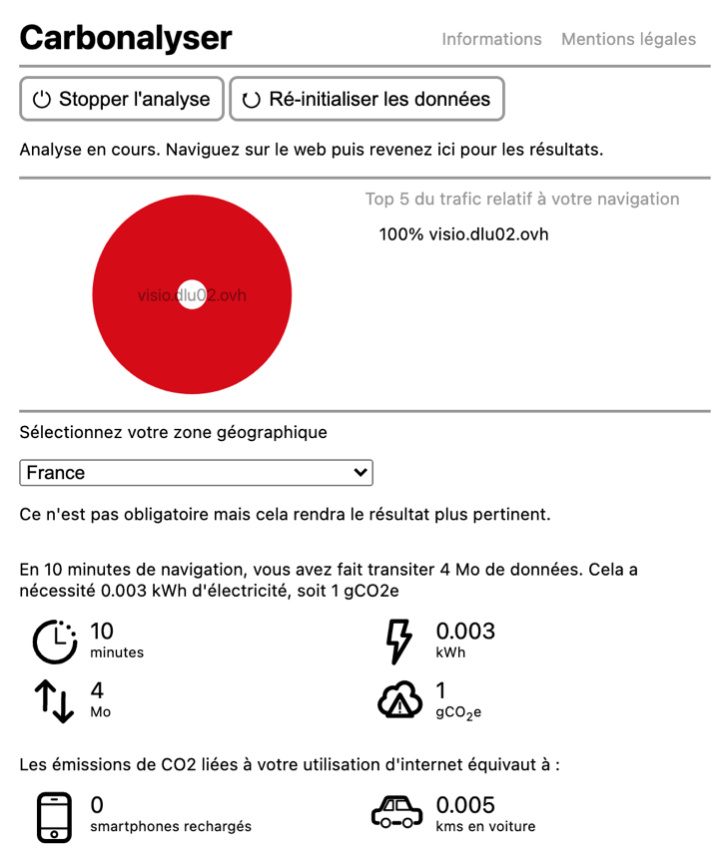
\includegraphics[scale=0.6]{mesure-jitsi-off.png}
\caption{Mesures obtenues sur une machine cliente avec Carbonalyser}
\end{figure}

et du côté du serveur hébergeant la conférence, on obtient avec powertop une valeur de 3.98W en moyenne

\section{Conclusion}

Pour la suite, il reste à mettre en oeuvre les scénarios présentés plus haut et à réaliser la synthèse des résultats pour établir une comparaison entre les différents outils (notamment sous forme de graphique ou de tableau).


\end{document}
 